\begin{frame}
\frametitle{Implementazione Hybrid Covert Channel}
Un Covert Channel ibrido è stato implementato combinando le tre tipologie di Covert Channel usate 
precedentemente: 
\begin{itemize}
    \item \textit{Timing Channel}: un byte indicherà il delay fra un pacchetto e l'altro. 
    \item \textit{Behavioural Channel}: da un byte verranno ricavate le due tipologie di messaggi da mandare. 
    \item \textit{Storage Channel}: in ciascun pacchetto verranno inseriti 
    tanti dati quanto la sua capacità di trasmissione. 
\end{itemize}  
La comunicazione viene iniziata tramite un messaggio \textit{Information Request} e chiusa sempre da un messaggio dello stesso tipo. 
\vspace{2ex}  \newline
Il destinatario, per ricevere i dati, monitora il flusso dei pachetti nella 
rete per rilevare l'intervallo di tempo con cui arrivano le coppie di messaggi. 
Da questo si ricaverà il byte relativo al tempo. Dalla coppia di messaggi 
ricava i quattro bit associati a ciascun messaggio. Dall'unione dei bit 
ricaverà il byte relativo alla tipologia di messaggi inviati. Ora non resta 
che ricavare i dati che sono stati nasconsti nei campi dei messaggi ICMP ricevuti.
\end{frame}
\begin{frame}
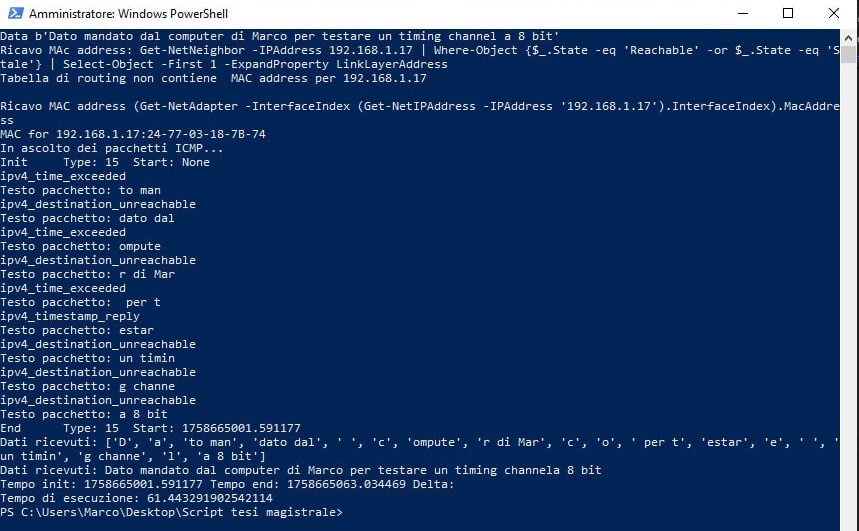
\includegraphics[width=\textwidth]{../Tesi/img/hybrid_channel/receiver_hybridChannel.jpg}
\captionof{figure}{Ricezione dei dait tramite Hybrid Covert Channel} 
\end{frame}

